%------------------------ Packages ------------------------
\documentclass[12pt,a4paper]{article}
\usepackage[latin1]{inputenc}
\usepackage[T1]{fontenc}
\usepackage[pdftex]{graphicx}
\usepackage{float}
\usepackage{amsmath}
\usepackage{amssymb}
\usepackage[FIGTOPCAP]{subfigure}
\usepackage{color}
\usepackage[hidelinks]{hyperref}

\newcommand{\version}{\IfFileExists{../../version.txt}
{\input{../../version.txt}}
{\input{../../../version.txt}}
}

\newcommand{\command}[1]{%
\indent \fcolorbox{black}{white}{%
   \begin{minipage}{\dimexpr\textwidth-\parindent\relax}%
      #1
   \end{minipage}%
}
}

\newsavebox{\FVerbBox}
\newenvironment{sample}
{\par \vspace{0.2cm} \begin{lrbox}{\FVerbBox}
\begin{minipage}{\dimexpr\textwidth-\parindent\relax}}
{\end{minipage}
\end{lrbox}
\fcolorbox{black}{lightgray}{\usebox{\FVerbBox}}
\vspace{0.2cm}}

\newenvironment{sampletitle}
{\vspace{0.2cm} \noindent\textbf{Example} :
\begin{sample}}
{\end{sample}}

\newcommand{\samplecomment}[1]{%

\textit{#1}
}

\newcommand{\seealso}[1]{\vspace{0.2cm} \noindent\textbf{See also} :\par #1}

% tikz
\usetikzlibrary{calc}
\usetikzlibrary{arrows}
\usetikzlibrary{shadows}

\tikzset{block/.style={draw, text centered, fill=gray!10,drop shadow}}
\tikzset{connect/.style={draw, line width=1 pt}}

\begin{document}

\begin{center}
\textbf{\huge  \underline{FAST algorithm for corner detection}}
\end{center}
\vspace{0.5cm}


FAST algorithm is used to detect corner in a image in real-time. FAST algorithm is proposed by Edward Rosten and Tom Drummond in their paper [1] (all images are taken from this paper).\\

\vspace{0.5cm} 


\begin{figure}[h!]
\centering
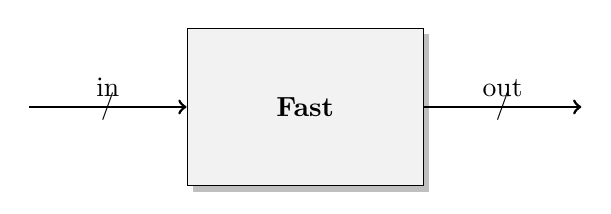
\begin{tikzpicture}
\node[block,rectangle,minimum height=2cm,minimum width=3cm] (bloc) {\textbf{Fast}};

\path[connect,<-] ([yshift=0.0cm]bloc.west) -- node{/} node[above]{in} ++(-2cm,0);

\path[connect,->] ([yshift=0.0cm]bloc.east) -- node{/} node[above]{out} ++(2cm,0);
 ([xshift=0.5cm,yshift=-0.6cm]bloc.north);

\end{tikzpicture}
\end{figure}

\vspace{1.5cm}

On the follow picture, we see the result of the FAST algorithm.\\

\begin{figure}[!h]
\centering
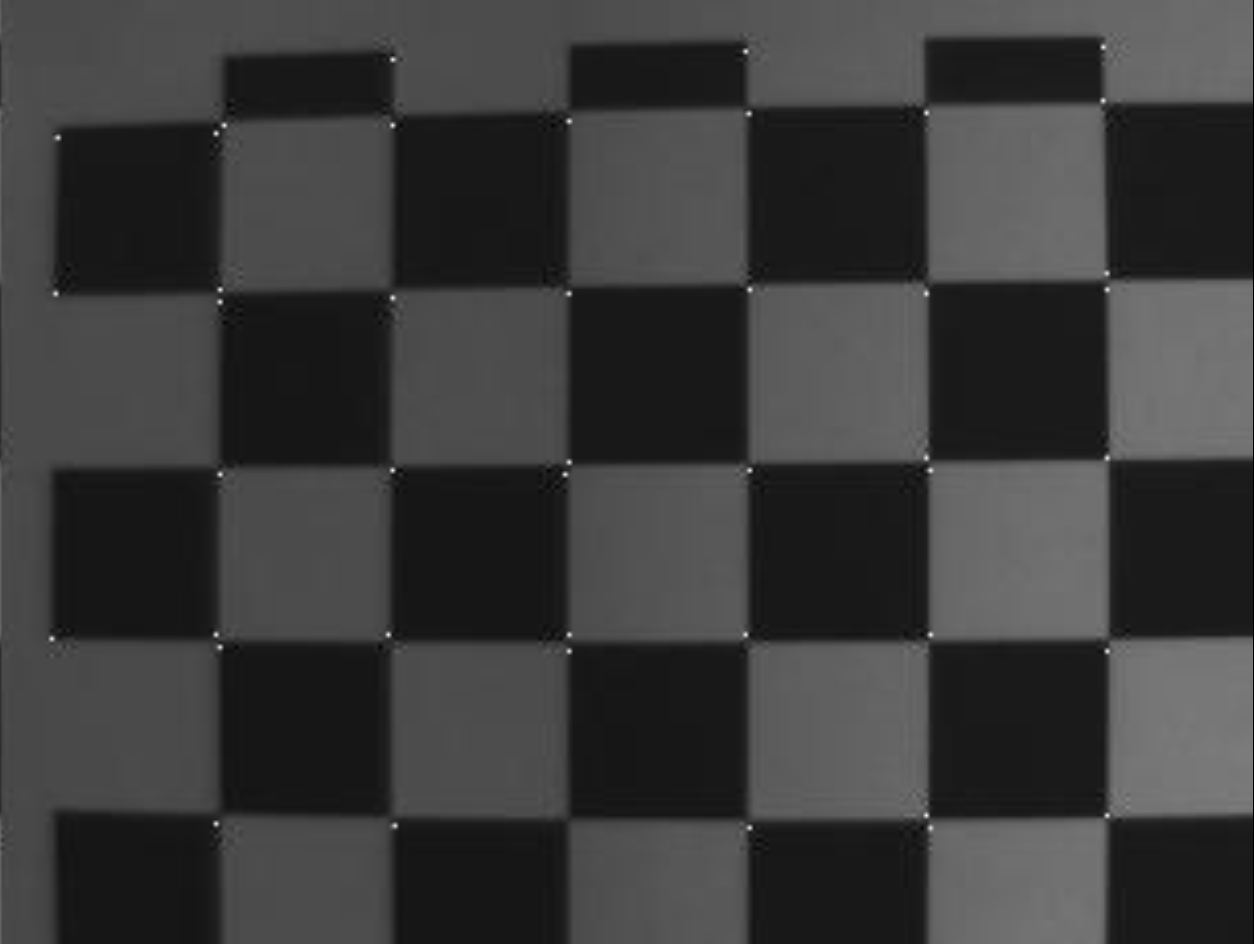
\includegraphics[width=5cm]{res.png}
\caption{Fast - Corner detection}
\end{figure}

\vspace{1.5cm}

\section*{Properties}
\properties{
enable & bool & Enable the processing \\ 
}

\newpage

\section*{Equivalence}
\subsection*{Matlab}

\lstset{language=Matlab}
\begin{lstlisting}
I = imread('yourimage.jpg');
I = rgb2gray(I);
corners = detectFASTFeatures(I);
imshow(I); hold on;
plot(corners.selectStrongest(50));
\end{lstlisting}

\url{https://nl.mathworks.com/help/vision/ref/detectfastfeatures.html}


\subsection*{OpenCV}

\lstset{language=C++}
\begin{lstlisting}
import numpy as np
import cv2
from matplotlib import pyplot as plt

img = cv2.imread('simple.jpg',0)

# Initiate FAST object with default values
fast = cv2.FastFeatureDetector()

# find and draw the keypoints
kp = fast.detect(img,None)
img2 = cv2.drawKeypoints(img, kp, color=(255,0,0))

# Print all default params
print "Threshold: ", fast.getInt('threshold')
print "nonmaxSuppression: ", fast.getBool('nonmaxSuppression')
print "neighborhood: ", fast.getInt('type')
print "Total Keypoints with nonmaxSuppression: ", len(kp)

cv2.imwrite('fast_true.png',img2)

\end{lstlisting}

\newpage

\section*{Explanation of the FAST Algorithm\footnote{http://docs.opencv.org/3.0-beta/doc/py\_tutorials/py\_feature2d/py\_fast/py\_fast.html}}

\begin{enumerate}
\item Select a pixel $p$ in the image which is to be identified as an interest point or not. Let its intensity be $I_p$.
\item Select appropriate threshold value $t$.
\item Consider a circle of 16 pixels around the pixel under test.

\begin{figure}[!h]
\centering
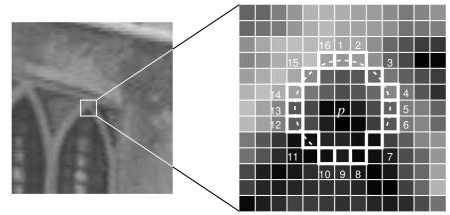
\includegraphics[width=10cm]{fast_expl.png}
\end{figure}

\item Now the pixel $p$ is a corner if there exists a set of n contiguous pixels in the circle (of 16 pixels) which are all brighter than $I_p+t$ or all darker than $I_p+t$. $n$ was chosen to be 12.

\item A high-speed test was proposed to exclude a large number of non-corners. This test examines only the four pixels at 1, 9, 5 and 13 (First 1 and 9 are tested if they are too brighter or darker. If so, then checks 5 and 13). If p is a corner, then at least three of these must all be brighter than $I_p+t$ or darker than $I_p-t$. If neither of these is the case, then p cannot be a corner. The full segment test criterion can then be applied to the passed candidates by examining all pixels in the circle. This detector in itself exhibits high performance, but there are several weaknesses : 

\end{enumerate}

\begin{figure}[!h]
\centering
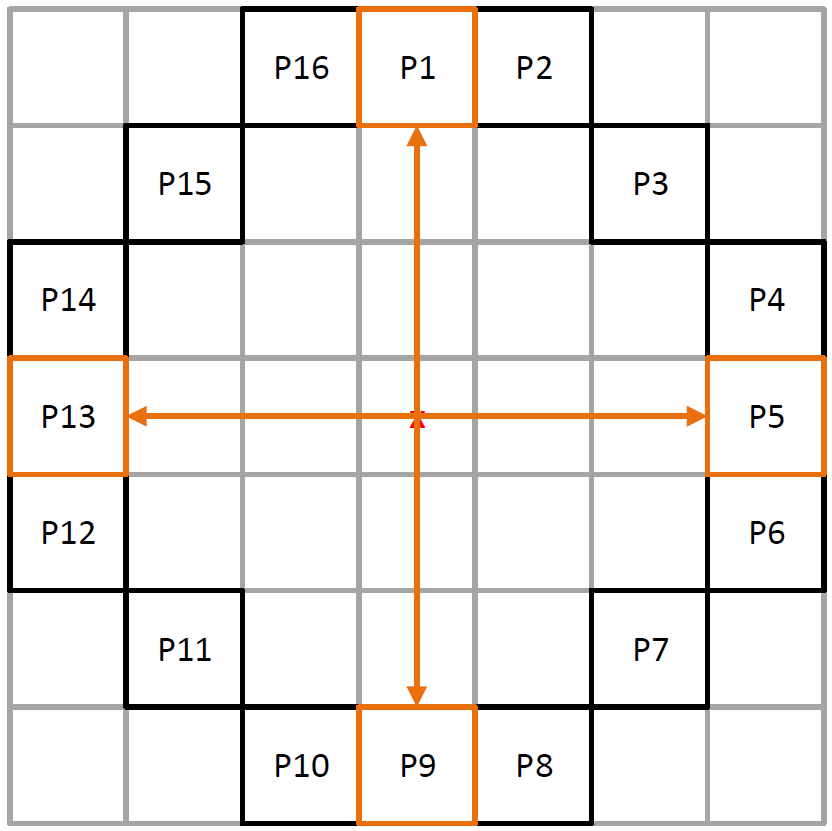
\includegraphics[width=5cm]{fast1.png}
\end{figure}


\newpage

after this, let's applying a filter to decrease the number of corner candidates. The full project on GPStudio is shown on the follow figure.  \\


\begin{figure}[!h]
\centering
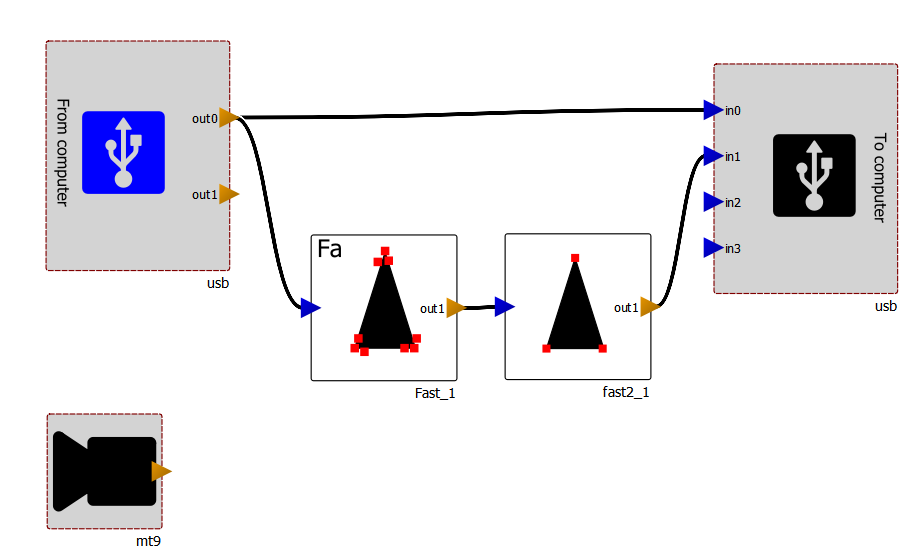
\includegraphics[width=10cm]{fast_filter.png}
\end{figure}


\end{document}